\documentclass{article}
\usepackage{geometry}
 \geometry{
 a4paper,
 total={170mm,270mm},
 left=20mm,
top=10mm,
 }
\usepackage{graphicx}
\usepackage{float}
\usepackage{enumitem}
\usepackage{caption}
\usepackage{amsmath}
\usepackage{datetime}
\usepackage{multirow}
\usepackage{listings}
\usepackage{amssymb}

\newcommand\blfootnote[1]{%
  \begingroup
  \renewcommand\thefootnote{}\footnote{#1}%
  \addtocounter{footnote}{-1}%
  \endgroup
}
\newcommand*{\addheight}[2][.5ex]{%
  \raisebox{0pt}[\dimexpr\height+(#1)\relax]{#2}%
}
\newdate{date}{15}{11}{2016}
\date{\displaydate{date}}
\title{\textbf{Network Analysis and Modelling - CSCI 5352} \\
Problem Set 6}
\author{\textbf{Santhanakrishnan Ramani}}
\begin{document}
\maketitle

\section*{Problem 1}
\blfootnote{Collaborated with Ruhi Saraf. Discussed about the problems after trying all by myself first.}
\begin{enumerate}[label=(\alph*)]
\item
The figure below shows the loglog plot of the ccdf of $Pr(K \geq k_{in})$ for network in-degree $k_{in}$ for value of $r={1,2,3,4}$ obtained by simulating the algorithm described in chapter 14.1.1 of Networks with value of $c=3$ and $n=10^6$.

\begin{table}[H]
\centering
\begin{tabular}{|c|c|}
	\hline
	\addheight{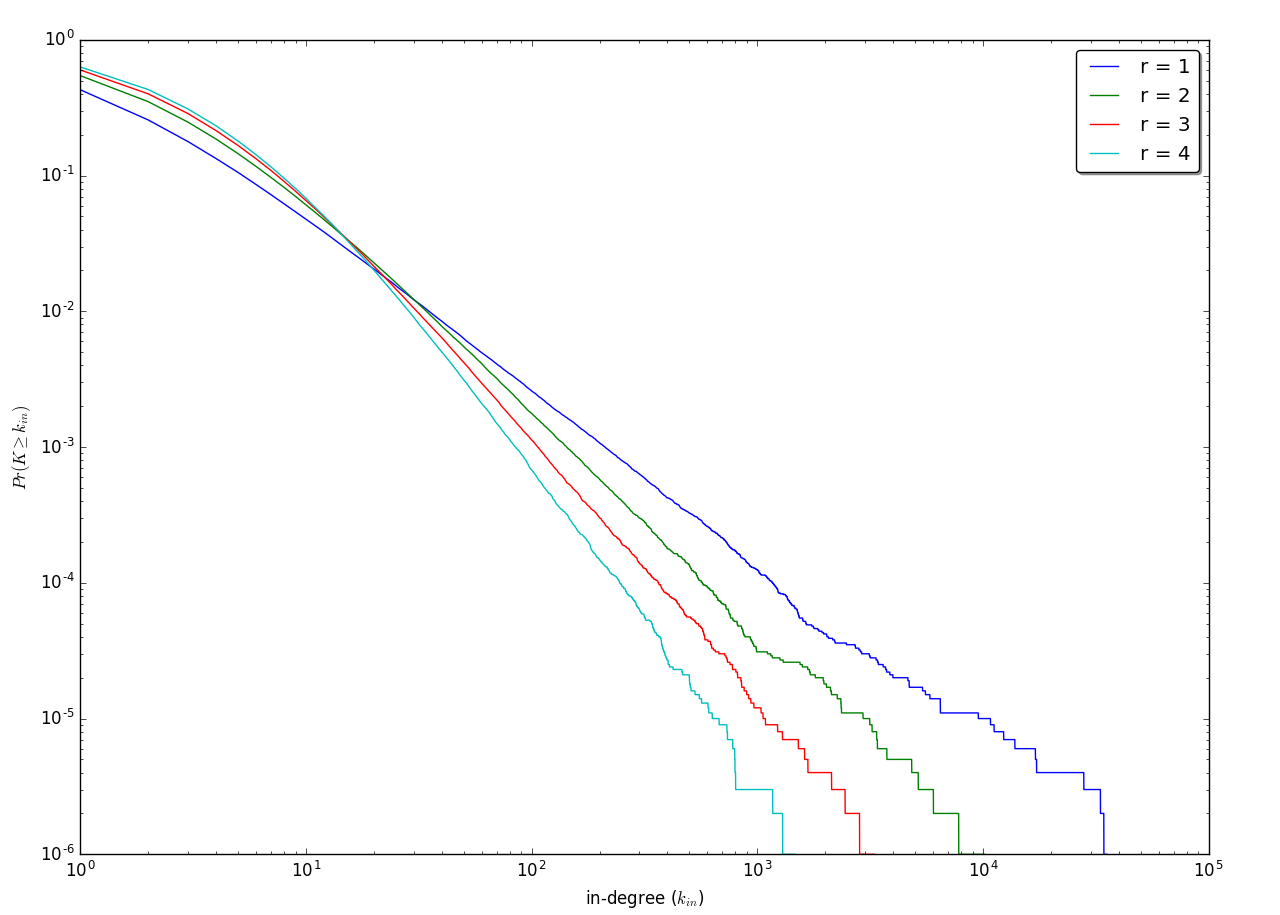
\includegraphics[width=100mm]{images/1a.png}} \\
	\hline
\end{tabular}
\end{table}

It's clear from the plot above that the distribution shape is similar to a power law distribution. As the probability of choosing from preferential attachment decreases with increase in the value of $r$, we can see that the value of maximum in-degree a node in the network can contain starts to decrease. There are many nodes having in-degree less than 50 compared to nodes containing higher in-degrees, the reason for the latter can attributed to the preferential attachment as the node with a higher in-degree are more likely to connected, while the reason for the former can be attributed to the nodes picked uniformly at random. We also see that the plots for different values of $r$ cross over each other when the in-degree is around 50 and the same probability, suggesting us that the number of nodes having in-degree greater than 50 is same for different values of $r$. The fraction of vertices with $k_{in} = 0$ is $57\%,\,45.5\%,\,40\%,\,36.8\%$ for values $r = 1,2,3,4$, so as the probability of uniform attachment increases the number of nodes with zero in-degree decreases as the chance to get picked increases.

\item
Using the parameters $c=12$ and $r=5$ that are considered reasonable values of the model parameters for real citation networks and averaging them over 200 iterations of the numerical simulation,
\begin{itemize}
\item
The average number of citations to a paper in the first $10\%$ of published papers is \textbf{81.3222568}
\item
The average number of citations to a paper in the last $10\%$ of published papers is \textbf{0.1871714}
\end{itemize}

From the values above we can clearly see the first-mover advantage in play. The comparatively larger average number of citations and bias for the first 10\% of the published papers over the last 10\% of the published paper can be attributed to the fact that a newly published paper cites a previously published paper using preferential attachment with a probability of 0.7. As a result the first published papers will start accumulating more connections and will be more likely to get connected than newly published papers.
 
\item
Using the hep-ph citation network,
\begin{itemize}
\item
The average in-degree of the first $10\%$ papers sorted based on submission date is \textbf{22.727}
\item
The average in-degree of the last $10\%$ papers sorted based on submission date is \textbf{5.8831}
\end{itemize} 

The empirical values obtained above agree with model estimates in (1b). We see the first-mover advantage but don't see too much of a bias for the first 10\% of the published papers over the last 10\% as we would expect as the total number of nodes in the network is only around 30000 and the slightly higher average for the last 10\% of the published papers due to the fact that new papers tend to cite more recent ones compared to the ones published long before.

\item
Below are the ways when Price's model of "preferential attachment" mechanism is considered unrealistic in modelling how nodes in a citation network accumulate new connections.
\begin{itemize}
\item
When your citation network is collection of papers from a certain domain for the past 100 years, you can see that the most recent papers will not be citing very old papers as the science would have advanced over years and they will be citing the papers which are 10-20 yrs old. Here it would be hard to differentiate the first-mover advantage as if some new technology boomed in this domain in the late years, the papers relating to it will be having more citations compared to the ones that came before that.
\item
When your citation network is collection of papers from different domain, in general papers from a certain domain will be most likely citing papers from that particular domain. So say some new domain like neural networks popped out in recent years and has a lots of publication we wouldn't see the same distribution as expected.  
\item
Nowadays, citations are random, because you search for something and end up citing it or you read some paper suggested by a peer or if you are a part of research group, you cite papers published by the group. The distribution of these kind of network's in-degree will look more like uniform distribution than power law as you choose random papers, and you can see lots of triangles in these network.
\end{itemize}

\item
The figure below shows us the loglog plot of the ccdfs for both the variation of Price's model where we remove the preferential attachment part and Price's model with parameters $c=3$ and $r={1,4}$.
\begin{table}[H]
\centering
\begin{tabular}{|c|c|}
	\hline
	\addheight{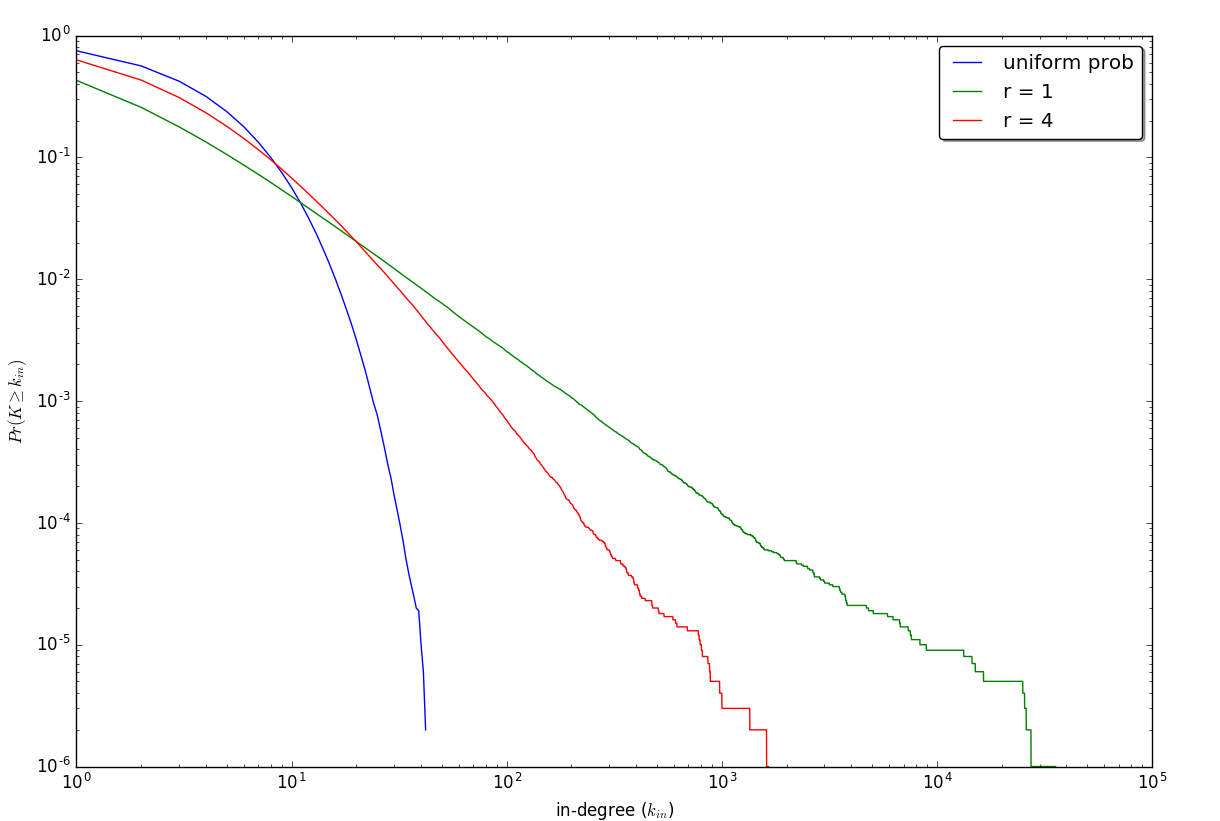
\includegraphics[width=100mm]{images/1e.png}} \\
	\hline
\end{tabular}
\end{table}
\end{enumerate}

From the plot above, we can see the number of nodes having $k_{in} = 0$ while using the variation model is only 25\% which is less compared to the price's model with 57\%. The maximum in-degree a node has in the variation model is only around 50 which is comparatively less to the ones achieved using price's model which are around 50000 and 2000 for values of $r=1,4$. The reason for the low value in the variation model is because all nodes are chosen uniformly at random. We can see that the variation model distribution doesn't follow power law and similar to price's model we can see large number of nodes having smaller in-degree.
 
\newpage
\section*{Code for Problem 1a}
\begin{lstlisting}[language=Python, breaklines=true] 
from __future__ import division
import random
import math
import numpy as np
import matplotlib.pyplot as plt
from collections import defaultdict

c = 3
n = 1000000
ccdf_dict = defaultdict(list)

for r in [1, 2, 3, 4]:
    print str(r)
    print "Initializing"
    p = c/(c+r)
    in_degree_cnt_list = np.zeros(n+1, dtype=np.int)
    in_degree_cnt_list[0] = -1
    in_degree_cnt_list[1:(c+1)] = c
    
    vertex_label_list = []
    for j in range(1, c+2):
        vertex_label_list.extend([j]*c)

    print "Price's Model simulation"
    for i in range(c+2, n+1):
        nodes = set()
        while len(nodes) < c:
            if random.random() < p:
                nodes.add(vertex_label_list[int(math.floor(c*(i-1)*random.random()))])
            else:
                nodes.add(int(math.ceil((i-1)*random.random())))
        vertex_label_list.extend(nodes)
        for node in nodes:
            in_degree_cnt_list[node] += 1
    
    print "Calculating ccdf"
    sorted_list = np.sort(in_degree_cnt_list)
    counts, bin_edges = np.histogram(sorted_list[1:], bins=range(0, max(sorted_list)+1))

    ccdf = np.zeros(len(counts), dtype=np.int)
    ccdf[0] = sum(counts)
    for k in range(1, len(counts)):
        ccdf[k] = ccdf[k-1] - counts[k-1]
    
    ccdf = [x/n for x in ccdf]
    ccdf_dict[r] = ccdf        

for r in ccdf_dict.keys():
    plt.plot(ccdf_dict[r], label="r = " + str(r))

plt.legend(loc='upper right', fancybox=True, shadow=True)
plt.tight_layout()
plt.yscale('log')
plt.xscale('log')
plt.xlabel(r'in-degree ($k_{in}$)')
plt.ylabel(r'$Pr(K \geq k_{in})$')
plt.show()
\end{lstlisting}

\newpage
\section*{Code for Problem 1b}
\begin{lstlisting}[language=Python, breaklines=true]
from __future__ import division
import random
import math
import numpy as np
from collections import defaultdict

c = 12
r = 5
n = 1000000
no_of_iter = 200
ccdf_dict = defaultdict(list)

avg_first_10 = 0
avg_last_10 = 0

for itr in range(no_of_iter):
    print str(itr)
    print "Initializing"
    p = c/(c+r)
    in_degree_cnt_list = np.zeros(n+1, dtype=np.int)
    in_degree_cnt_list[0] = -1
    in_degree_cnt_list[1:(c+1)] = c
    
    vertex_label_list = []
    for j in range(1, c+2):
        vertex_label_list.extend([j]*c)

    print "Price's Model simulation"
    for i in range(c+2, n+1):
        nodes = set()
        while len(nodes) < c:
            if random.random() < p:
                nodes.add(vertex_label_list[int(math.floor(c*(i-1)*random.random()))])
            else:
                nodes.add(int(math.ceil((i-1)*random.random())))
        vertex_label_list.extend(nodes)
        for node in nodes:
            in_degree_cnt_list[node] += 1
    
    print "Calculating average"
    avg_first_10 += sum(in_degree_cnt_list[:100000])/100000
    avg_last_10 += sum(in_degree_cnt_list[-100000:])/100000    

print avg_first_10/no_of_iter
print avg_last_10/no_of_iter
\end{lstlisting}

\newpage
\section*{Code for Problem 1c}
\begin{lstlisting}[language=Python, breaklines=true]
from __future__ import division
import operator
import networkx as nx
from collections import defaultdict

dataPath = "/home/santa/Dropbox/NAM/Problem Set 6/data/"
filename1 = 'Cit-HepPh.txt'
filename2 = 'cit-HepPh-dates.txt'

lines = [line.rstrip('\n') for line in open(dataPath+filename1)]
G = nx.DiGraph()
for line in lines:
    vertexes = line.split("\t")
    G.add_edge(int(vertexes[0]), int(vertexes[1]))
    
lines = [line.rstrip('\n\r') for line in open(dataPath+filename2)]
date_map = defaultdict()
for line in lines:
    node_id, date = line.split("\t")
    date_map[int(node_id)] = date

sorted_date_map = sorted(date_map.items(), key=operator.itemgetter(1))
tenPC = int(len(sorted_date_map)/10)

avg_first_10 = 0
avg_last_10 = 0

nodes = G.nodes()
for tup in sorted_date_map[:tenPC]:
    if tup[0] in nodes:
        avg_first_10 += G.in_degree(tup[0])

for tup in sorted_date_map[-tenPC:]:
    if tup[0] in nodes:
        avg_last_10 += G.in_degree(tup[0])

print avg_first_10/tenPC
print avg_last_10/tenPC 
\end{lstlisting}
\hspace{5mm}
\section*{Code for Problem 1e}
\begin{lstlisting}[language=Python, breaklines=true]
from __future__ import division
import random
import math
import numpy as np
import matplotlib.pyplot as plt
from collections import defaultdict

c = 3
n = 1000000

print "Initializing"
in_degree_cnt_list = np.zeros(n+1, dtype=np.int)
in_degree_cnt_list[0] = -1
in_degree_cnt_list[1:(c+1)] = c

print "Variation of Price's Model simulation"
for i in range(c+2, n+1):
    nodes = set()
    while len(nodes) < c:
        nodes.add(int(math.ceil((i-1)*random.random())))
    for node in nodes:
        in_degree_cnt_list[node] += 1

print "Calculating ccdf"
sorted_list = np.sort(in_degree_cnt_list)
[counts, bin_edges] = np.histogram(sorted_list[1:], bins=range(0, max(sorted_list) + 1))
ccdf = np.zeros(len(counts), dtype=np.int)
ccdf[0] = sum(counts)
for k in range(1, len(counts)):
    ccdf[k] = ccdf[k-1] - counts[k-1]
ccdf = [x/n for x in ccdf]
plt.plot(ccdf, label='uniform prob')


ccdf_dict = defaultdict(list)
for r in [1, 4]:
    print str(r)
    print "Initializing"
    p = c/(c+r)
    in_degree_cnt_list = np.zeros(n+1, dtype=np.int)
    in_degree_cnt_list[0] = -1
    in_degree_cnt_list[1:(c+1)] = c
    
    vertex_label_list = []
    for j in range(1, c+2):
        vertex_label_list.extend([j]*c)

    print "Price's Model simulation"
    for i in range(c+2, n+1):
        nodes = set()
        while len(nodes) < c:
            if random.random() < p:
                nodes.add(vertex_label_list[int(math.floor(c*(i-1)*random.random()))])
            else:
                nodes.add(int(math.ceil((i-1)*random.random())))
        vertex_label_list.extend(nodes)
        for node in nodes:
            in_degree_cnt_list[node] += 1
    
    print "Calculating ccdf"
    sorted_list = np.sort(in_degree_cnt_list)
    [counts, bin_edges] = np.histogram(sorted_list[1:], bins = range(0, max(sorted_list) + 1))
    ccdf = np.zeros(len(counts), dtype=np.int)
    ccdf[0] = sum(counts)
    for k in range(1, len(counts)):
        ccdf[k] = ccdf[k-1] - counts[k-1]
    ccdf = [x/n for x in ccdf]
    ccdf_dict[r] = ccdf        

for r in ccdf_dict.keys():
    plt.plot(ccdf_dict[r], label='r = '+str(r))

plt.legend(loc='upper right', fancybox=True, shadow=True)
plt.tight_layout()
plt.yscale('log')
plt.xscale('log')
plt.xlabel(r'in-degree ($k_{in}$)')
plt.ylabel(r'$Pr(K \geq k_{in})$')
plt.show()
\end{lstlisting}
\end{document}
